%%%%%%%%%%%%%%%%%%%%%%%%%%%%%%%%%%%%%%%%%
% Journal Article
% LaTeX Template
% Version 1.4 (15/5/16)
%
% This template has been downloaded from:
% http://www.LaTeXTemplates.com
%
% Original author:
% Frits Wenneker (http://www.howtotex.com) with extensive modifications by
% Vel (vel@LaTeXTemplates.com)
%
% License:
% CC BY-NC-SA 3.0 (http://creativecommons.org/licenses/by-nc-sa/3.0/)
%
%%%%%%%%%%%%%%%%%%%%%%%%%%%%%%%%%%%%%%%%%

%----------------------------------------------------------------------------------------
%	PACKAGES AND OTHER DOCUMENT CONFIGURATIONS
%----------------------------------------------------------------------------------------

\documentclass[twoside,twocolumn]{article}

\usepackage{blindtext} % Package to generate dummy text throughout this template 

\usepackage[sc]{mathpazo} % Use the Palatino font
\usepackage[T1]{fontenc} % Use 8-bit encoding that has 256 glyphs
\linespread{1.05} % Line spacing - Palatino needs more space between lines
\usepackage{microtype} % Slightly tweak font spacing for aesthetics
\usepackage{float}
\usepackage{graphicx}


\usepackage[english]{babel} % Language hyphenation and typographical rules

\usepackage[hmarginratio=1:1,top=32mm,columnsep=20pt]{geometry} % Document margins
\usepackage[hang, small,labelfont=bf,up,textfont=it,up]{caption} % Custom captions under/above floats in tables or figures
\usepackage{booktabs} % Horizontal rules in tables

\usepackage{lettrine} % The lettrine is the first enlarged letter at the beginning of the text

\usepackage{enumitem} % Customized lists
\setlist[itemize]{noitemsep} % Make itemize lists more compact

\usepackage{abstract} % Allows abstract customization
\renewcommand{\abstractnamefont}{\normalfont\bfseries} % Set the "Abstract" text to bold
\renewcommand{\abstracttextfont}{\normalfont\small\itshape} % Set the abstract itself to small italic text

\usepackage{titlesec} % Allows customization of titles
\renewcommand\thesection{\Roman{section}} % Roman numerals for the sections
\renewcommand\thesubsection{\roman{subsection}} % roman numerals for subsections
\titleformat{\section}[block]{\large\scshape\centering}{\thesection.}{1em}{} % Change the look of the section titles
\titleformat{\subsection}[block]{\large}{\thesubsection.}{1em}{} % Change the look of the section titles

\usepackage{fancyhdr} % Headers and footers
\pagestyle{fancy} % All pages have headers and footers
\fancyhead{} % Blank out the default header
\fancyfoot{} % Blank out the default footer
\fancyhead[C]{Seminar Data Science \& Artificial Intelligence $\bullet$ SS25} % Custom header text
\fancyfoot[RO,LE]{\thepage} % Custom footer text

\usepackage{titling} % Customizing the title section

\usepackage{hyperref} % For hyperlinks in the PDF

\usepackage[acronym]{glossaries}
\makeglossaries

\newacronym{SAC}{SAC}{Soft Actor Critic}
\newacronym{DDPG}{DDPG}{Deep Deterministic Policy Gradient}
\newacronym{PPO}{PPO}{Proximal Policy Optimization}
\newacronym{RL}{RL}{einforcement learning}
\newacronym{SB3}{SB3}{Stable Baselines 3}



%----------------------------------------------------------------------------------------
%	TITLE SECTION
%----------------------------------------------------------------------------------------

\setlength{\droptitle}{-4\baselineskip} % Move the title up

\pretitle{\begin{center}\Huge\bfseries} % Article title formatting
\posttitle{\end{center}} % Article title closing formatting
\title{Continuous Control in Reinforcement Learning} % Article title
\author{%
\textsc{Leonard Kreil \& Zia A. J. Asmara} \\[1ex] % Your name
\normalsize Wedel University of Applied Sciences\\ % Your institution
\normalsize \href{stud106680@fh-wedel.de}{stud106680@fh-wedel.de} \\ % Your email address
\normalsize \href{stud106700@fh-wedel.de}{stud106700@fh-wedel.de} % Your email address
%\and % Uncomment if 2 authors are required, duplicate these 4 lines if more
%\textsc{Jane Smith}\thanks{Corresponding author} \\[1ex] % Second author's name
%\normalsize University of Utah \\ % Second author's institution
%\normalsize \href{mailto:jane@smith.com}{jane@smith.com} % Second author's email address
}
\date{\today} % Leave empty to omit a date
\renewcommand{\maketitlehookd}{%
\begin{abstract}
\noindent This paper provides an overview of continuous control in reinforcement learning and compares three prominent algorithms: \gls{DDPG}, \gls{PPO}, and \gls{SAC}. Using OpenAI Gym's BipedalWalker-v3 environment, we evaluate these algorithms without hyperparameter tuning. \gls{SAC} demonstrates superior performance, while \gls{PPO} shows faster training but slower convergence, and \gls{DDPG} underperforms with significant instability. For complex continuous control tasks with limited tuning capacity, \gls{SAC} proves most suitable for real-world robotics applications due to its robust performance and sample efficiency.
\end{abstract}
}

%----------------------------------------------------------------------------------------

\begin{document}

% Print the title
\maketitle
%----------------------------------------------------------------------------------------
%	ARTICLE CONTENTS
%----------------------------------------------------------------------------------------
\section{Introduction}

\lettrine[nindent=0em,lines=3]{R} \MakeLowercase{\gls{RL}} has achieved remarkable successes across various domains, from games like Go and chess~\cite{doi:10.1126/science.aar6404} to industrial processes ~\cite{NEURIPS2018_059fdcd9}. While discrete action spaces are well-studied, many real-world applications require agents to operate in continuous action spaces, which represents a more challenging domain known as continuous control ~\cite{lillicrap2019continuouscontroldeepreinforcement}. In continuous control, agents must select actions from an infinite set of possibilities rather than choosing from finite discrete options.\\

\noindent Continuous control has gained attention due to its direct applicability to robotics, autonomous vehicles, and physical systems that require precise control signals rather than discrete choices. For example, a walking robot needs specific joint torque values rather than simply "move forward" or "turn left" commands~\cite{lillicrap2019continuouscontroldeepreinforcement}.\\

\noindent This domain presents several fundamental challenges. First, exploration is more difficult as agents must search through infinite action spaces~\cite{duan2016benchmarkingdeepreinforcementlearning}. Second, function approximation becomes necessary for policies and value functions. Third, complex dynamics and long time horizons require learning long-term dependencies~\cite{lillicrap2019continuouscontroldeepreinforcement}.\\

\noindent The Bipedal Walker environment from OpenAI Gym demonstrates these challenges, which require an agent to control a two-legged robot to walk forward without falling. The robot must apply continuous torque values to each joint~\cite{openai2021bipedalwalker}. The task combines the challenges of balance and coordination, making it an excellent benchmark for comparing continuous control algorithms.\\

\noindent This paper compares three prominent continuous control algorithms, \gls{DDPG}~\cite{lillicrap2019continuouscontroldeepreinforcement}, \gls{PPO}~\cite{schulman2017proximalpolicyoptimizationalgorithms}, and \gls{SAC}~\cite{haarnoja2018softactorcriticoffpolicymaximum}, analyzing their performance, convergence properties, and stability characteristics using the Bipedal Walker environment.
%------------------------------------------------
\section{Theoretical foundations}

This chapter is primarily based on the presentation by Sutton and Barto~\cite{Sutton2018}\footnote{All definitions and concepts not attributed to other sources are based on the exposition in Sutton and Barto (2018).}.

\subsection{\gls{RL} for Continuous Control}

\newacronym{MDP}{MDP}{Markov Decision Process}
\subsubsection{\gls{MDP}}

\begin{figure}[H] % Use figure* for full-width in twocolumn
    \centering
    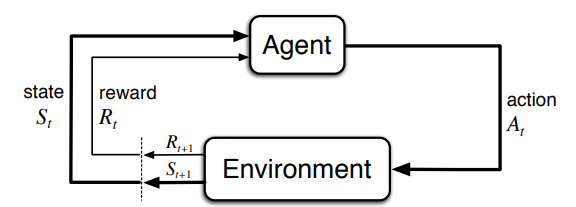
\includegraphics[width=0.45\textwidth]{MDP.png} % Passe den Dateinamen und Pfad an
    \caption{The agent environment interaction in a Markov decision process~\cite{Sutton2018}.}
    \label{fig:first} % For first figure
\end{figure}
\gls{RL} problems are typically formalized as \gls{MDP}s. An \gls{MDP} is defined by the tuple $(\mathcal{S}, \mathcal{A}, \mathcal{P}, \mathcal{R}, \gamma)$, where:

\begin{itemize}
    \item $\mathcal{S}$ is the state space,
    \item $\mathcal{A}$ is the action space,
    \item $\mathcal{P}$ is the transition probability distribution (or transition dynamics in the continuous case),
    \item $\mathcal{R}$ is the reward function,
    \item $\gamma \in [0,1]$ is the discount factor.
\end{itemize}

\noindent For continuous control problems, both $\mathcal{S}$ and $\mathcal{A}$ are continuous sets, typically represented as vectors of real values. Typically, the transition dynamics and reward functions are also continuous mappings. In continuous control, the transition dynamics are often described as a probability density over the next state.

\subsubsection{Agent, Environment, Reward and Policy}

Within this \gls{MDP}, \gls{RL} is considered in the context of an agent interacting with an environment over a sequence of time steps. This interaction can be formally described as shown in Figure~\ref{fig:first}:

\noindent At each time step~$t$:
\begin{itemize}
    \item The agent observes the current state $s_t \in \mathcal{S}$ of the environment,
    \item selects an action $a_t \in \mathcal{A}$ based on its policy,
    \item receives a reward $r_t \in \mathbb{R}$ from the environment, and
    \item transitions to a new state $s_{t+1}$.
\end{itemize}

\noindent The agent is the learning entity that aims to maximize the cumulative reward. It observes the environment through its state representation and acts according to its policy. Mathematically, the agent's objective is to maximize the expected return $G_t$, defined as the discounted sum of future rewards:

\begin{equation}
G_t = \sum_{k=0}^{\infty} \gamma^k r_{t+k+1}
\end{equation}

\noindent where $\gamma \in [0,1]$ is the discount factor, which determines the present value of future rewards.\\

\noindent The environment defines the dynamics of the system in which the agent operates. It determines how the state evolves and what reward is returned in response to the agent’s actions. Given a current state and an action taken by the agent, the environment produces the next state and the corresponding reward. This interaction captures the core feedback mechanism that enables learning in \gls{RL}.\\

\noindent The reward \( r_t \) is a scalar signal provided by the environment that indicates how good the agent’s action is in the current state. The reward function is formally defined as:

\begin{equation}
\mathcal{R}: \mathcal{S} \times \mathcal{A} \times \mathcal{S} \rightarrow \mathbb{R}
\end{equation}

\noindent where \( \mathcal{R}(s_t, a_t, s_{t+1}) \) represents the expected immediate reward when transitioning from state \( s_t \) to state \( s_{t+1} \) after taking action \( a_t \).\\

\noindent The policy \( \pi \) defines the agent’s strategy for selecting actions based on the current state. It guides the agent’s behavior by determining which action to take in each situation. In the case of a stochastic policy, \( \pi(a|s) \) represents the probability of taking action \( a \) given state \( s \). This allows the agent to explore different actions with varying likelihoods. For deterministic policies, the policy is a direct mapping from states to actions, written as:
\begin{equation} \pi(s) = a \end{equation}
Which means the agent always chooses the same action \( a \) in state \( s \).\\

\noindent The value function $V^\pi(s)$ represents the expected return when the agent starts in state $s$ and follows policy $\pi$:
\begin{equation} V^\pi(s) = \mathbb{E}_{\pi}\left[G_t \middle| S_t = s\right] \end{equation}
In continuous control problems the expectation is calculated over a continuous probability density of future states.\\

\noindent The action-value function $Q^\pi(s,a)$ represents the expected return when action $a$ is taken in state $s$ and policy $\pi$ is followed thereafter:
\begin{equation} Q^\pi(s,a) = \mathbb{E}_{\pi}\left[G_t \middle| S_t = s, A_t = a\right] \end{equation}
In continuous control problems, $a$ is a vector of continuous actions. The action-value function accounts for the probability density of transitions.\\

\noindent The optimal policy $\pi^*$ maximizes the expected return in every state:
\begin{equation} \pi^* = \arg\max_\pi V^\pi(s) \quad \forall s \in \mathcal{S} \end{equation}
For continuous control, the definition of the optimal policy remains the same, but policy $\pi^*$ provides a continuous action recommendation in each state.

\subsubsection{Differences Between Discrete and Continuous Action Spaces}

The fundamental difference between discrete and continuous action spaces lies in the number of possible actions available to the agent.

\noindent Discrete action spaces have a finite number of actions from which the agent can choose:
\begin{equation}
    \mathcal{A} = \{a_1, a_2, ..., a_n\}
\end{equation}
Examples are selecting one of four directions in a grid world or selecting a move in chess.\\
\noindent Continuous action spaces have actions from an uncountably infinite set, typically represented as real-valued vectors:
\begin{equation}
\mathcal{A} \subseteq \mathbb{R}^d
\end{equation}
where $d$ is the dimensionality of the action space. Examples are controlling joint torques in a robotic arm or adjusting steering and acceleration in a vehicle.\\

\noindent This results in several differences in algorithm design:

\begin{itemize}
    \item Exploration strategies:  Discrete spaces can use simple methods like  $\varepsilon$-greedy or softmax policies, while continuous spaces require adding noise to actions (\gls{DDPG} \cite{lillicrap2019continuouscontroldeepreinforcement}) or using stochastic policies that model probability distributions over actions (\gls{SAC} \cite{haarnoja2018softactorcriticoffpolicymaximum}, \gls{PPO} \cite{schulman2017proximalpolicyoptimizationalgorithms}).
    \item Action selection: Discrete actions use argmax operations over Q-values, where continuous actions involve sampling from stochastic policies or directly outputting values through specialized policy networks.
    \item Function approximation: Continuous action spaces need more advanced techniques to represent policies and value functions across infinite action domains \cite{fujimoto2018addressingfunctionapproximationerror}.
\end{itemize}

\subsubsection{Policy Gradient Methods}

Policy gradient methods are especially well-suited for continuous control problems because they optimize the policy parameters directly, without needing to discretize the action space. The main idea is to adjust the parameters $\theta$ of a parameterized policy $\pi_\theta$ in the direction of the expected return gradient\cite{wang2019neural}:

\begin{equation}
\nabla_\theta J(\pi_\theta) = \mathbb{E}_{\sigma_{\pi_\theta}} \left[ Q^{\pi_\theta}(s, a) \cdot \nabla_\theta \log \pi_\theta(a \mid s) \right]
\end{equation}

\noindent This is known as the policy gradient theorem, where $J(\theta)$ represents the expected return under the policy $\pi_\theta$:

\begin{equation}
J(\theta) = \mathbb{E}_{\pi_\theta} \left[G_0\right]
\end{equation}

\noindent For continuous action spaces, the policy $\pi_\theta(a|s)$ is often modeled as a Gaussian distribution:

\begin{equation}
\pi_\theta(a|s) = \mathcal{N}(\mu_\theta(s), \sigma_\theta(s))
\end{equation}

\noindent Here, $\mu_\theta(s)$ and $\sigma_\theta(s)$ are the mean and standard deviation of the action distribution.

%\noindent Actor-critic methods combine policy gradient techniques with value function approximation. In this setup, an actor network learns the policy, while a critic network estimates the action values or advantages.

\subsection{Function Approximation in \gls{RL}}

In continuous control tasks, both the state and action spaces are continuous, making it impractical to represent value functions or policies using tabular methods. The function approximation, particularly with neural networks, has become the standard approach to manage the complexity and dimensionality in these problems~\cite{gottwald2018neuralvalue}.

\subsubsection{Neural Networks as Function Approximators}

Neural networks serve as universal function approximators, capable of modeling complex relationships between continuous states and actions. In continuous control settings, they are typically utilized in two primary roles:
\begin{itemize}
    \item Value function approximation: Neural networks estimate state value functions $V(s)$ or action value functions $Q(s, a)$, mapping continuous inputs to scalar outputs~\cite{gottwald2018neuralvalue}.
    \item Policy approximation: Networks directly parameterize policies, which can be:
    \begin{itemize}
        \item \textit{Deterministic:} Outputting specific continuous actions.
        \item \textit{Stochastic:} Outputting parameters of probability distributions over actions~\cite{gottwald2018neuralvalue}.
    \end{itemize}
\end{itemize}

\noindent The flexibility of neural networks allows them to capture non-linear dependencies, which makes them well suited for continuous control problems such as those found in robotics~\cite{gottwald2018neuralvalue}.

\subsubsection{Challenges in Representing Continuous Policies}

Representing policies in continuous action spaces introduces several unique challenges.
\begin{itemize}
    \item Output representation:  Neural networks must produce outputs within feasible ranges for each action dimension, enforced using bounded activation functions (e.g. \texttt{ tanh}) or by post-processing outputs~\cite{wang2018explorationexploitation}.
    \item Exploration-exploitation tradeoff: Exploration in continuous spaces relies on adding Gaussian noise to deterministic policies or sampling from learned stochastic policies~\cite{wang2018explorationexploitation}.
    \item Training stability: Minor parameter changes can lead to large behavioral differences, requiring techniques such as gradient clipping, target networks, and conservative policy updates to stabilize learning~\cite{shen2024ddpgtd3walker2d}.
\end{itemize}

\subsubsection{Actor-Critic Architecture Overview}

The actor-critic architecture is fundamental in modern continuous control algorithms. It comprises two interacting neural networks:

\begin{figure}[H] % Use figure* for full-width in twocolumn
    \centering
    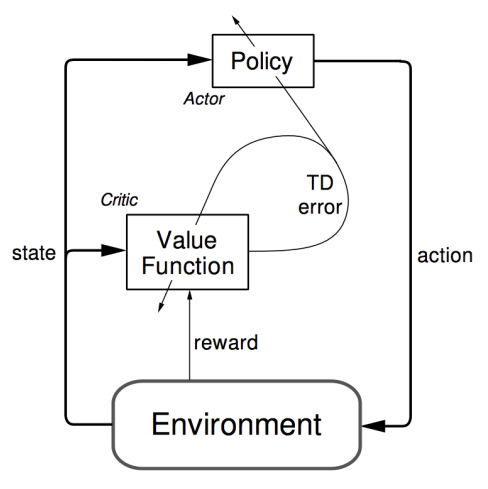
\includegraphics[width=0.45\textwidth]{actorcritic.png} % Passe den Dateinamen und Pfad an
    \caption{Scheme of information flows in actor-critic agent \cite{Sutton2018}.}
    \label{fig:mdp}
\end{figure}

\begin{itemize}
    \item Actor network: Represents the policy $\pi(a|s)$, mapping states to actions. For continuous actions, the actor typically outputs either: \begin{itemize}
        \item Mean and standard deviation for a Gaussian policy, or
        \item Direct deterministic action values.
    \end{itemize}
    \item Critic network: Estimates value functions, providing a learning signal to guide actor updates.
    %such as $Q(s, a)$ or the advantage function $A(s, a)$
\end{itemize}

\noindent This dual network system improves training stability compared to pure policy gradient methods. The critic reduces the variance of the gradient, while the actor allows efficient optimization of continuous actions~\cite{Sutton2018}. The actor-critic framework forms the basis for many state-of-the-art algorithms in continuous control, including \gls{DDPG}, \gls{PPO}, and \gls{SAC}, which we will examine in detail in the following section.


\section{Algorithms for Continuous Control}

\subsection{\gls{DDPG}}
\gls{DDPG}, introduced by Lillicrap et al.~\cite{lillicrap2019continuouscontroldeepreinforcement}, adapts the deterministic policy gradient by incorporating deep neural networks for function approximation. It is an off-policy, actor-critic algorithm designed for continuous action spaces.\\

\noindent \gls{DDPG} relies on the deterministic policy gradient theorem to compute gradients of the expected return with respect to the policy parameters \cite{lillicrap2019continuouscontroldeepreinforcement}:

{\footnotesize
\begin{equation}
\nabla_{\theta^\mu} J \approx \mathbb{E}_{s \sim \rho^\beta}\left[\nabla_a Q(s, a|\theta^Q)\big|_{a=\mu(s|\theta^\mu)} \cdot \nabla_{\theta^\mu} \mu(s|\theta^\mu)\right]
\end{equation}
}

\noindent where $\mu(s|\theta^\mu)$ is the deterministic policy, $Q(s, a|\theta^Q)$ is the action-value function, and $\rho^\beta$ is the state distribution under the behavior policy $\beta$.

\noindent The core components of \gls{DDPG}:

\begin{itemize}
    \item Deterministic Actor: Policy network $\mu_\theta(s)$ mapping states directly to actions.
    \item Q-Network Critic: Q-network estimating the action-value function $Q(s, a)$.
\end{itemize}

\noindent Stability mechanism:
\begin{itemize}
    \item Target Networks: Slowly updated copies, $\mu_{\theta'}$ and $Q_{\phi'}$, used for training stability.
    \item Replay Buffer: Stores transitions for sample-efficient learning.
    \item Exploration: Adds noise to deterministic actions \cite{lillicrap2019continuouscontroldeepreinforcement}:
    \begin{equation}
    a = \mu(s|\theta^\mu) + \mathcal{N}
    \end{equation}
    where $\mathcal{N}$ is typically Ornstein-Uhlenbeck or Gaussian noise.
\end{itemize}

\noindent \gls{DDPG} training alternates between environment interaction and network updates. The actor selects actions with added noise to encourage exploration, and the resulting transitions are stored in a replay buffer.\\

\noindent During the learning phase, mini-batches sampled from this buffer are used to update the critic by minimizing the Bellman error\footnote{The Bellman error measures the difference between predicted Q-values and the target values computed using the Bellman equation: $|Q(s,a) - (r + \gamma Q(s',a'))|$.}, and to update the actor by maximizing the predicted Q-values estimated by the critic.\\

\noindent To maintain training stability, target networks are slowly updated using Polyak averaging \cite{lillicrap2019continuouscontroldeepreinforcement}:
\begin{equation}
\theta' \leftarrow \tau \theta + (1 - \tau) \theta',
\end{equation}
\noindent where \(\tau \ll 1\) controls the smoothness of the update.\\

\noindent This approach offers several advantages, including high sample efficiency due to off-policy learning and a relatively straightforward implementation. However, it also comes with limitations, such as sensitivity to hyperparameter settings and noise configuration, as well as potential training instability in more complex environments~\cite{lillicrap2019continuouscontroldeepreinforcement}.


\subsection{\gls{PPO}}

Introduced by Schulman et al.~\cite{schulman2017proximalpolicyoptimizationalgorithms}, \gls{PPO} is a policy gradient method designed to address the instability often encountered in earlier policy optimization approaches. \gls{PPO} is an on-policy and excels in discrete and continuous action spaces, balancing stability and simplicity.\\

\noindent \gls{PPO}'s key innovation is its clipping mechanism that prevents excessive policy updates and improves training stability. The clipped objective function is formulated as \cite{schulman2017proximalpolicyoptimizationalgorithms}:

{\footnotesize
\begin{equation}
L^{\text{CLIP}}(\theta) = \mathbb{E}_t\left[\min\left(r_t(\theta)\hat{A}_t,\ \text{clip}(r_t(\theta), 1 - \epsilon, 1 + \epsilon)\hat{A}_t\right)\right]
\end{equation}
}

\noindent where \(r_t(\theta) = \frac{\pi_\theta(a_t|s_t)}{\pi_{\theta_{\text{old}}}(a_t|s_t)}\) is the probability ratio between the new and old policies, \(\hat{A}_t\) is the estimated advantage function, \(\epsilon\) is a hyperparameter (typically 0.1 or 0.2) that defines the clipping range.\\

\noindent The core components of \gls{PPO} are:
\newacronym{GAE}{GAE}{Generalized Advantage Estimation}
\begin{itemize}
    \item Stochastic Policy Network \(\pi_\theta\): Determines action probabilities.
    
    \item Value Network \(V_\phi\): Estimates expected rewards (state-value function).
    
    \item Advantage Estimation: Helps the agent figure out how much better an action is compared to the average. It uses \gls{GAE}.
    
    \item Clipped Objective: Limits policy updates to ensure training stability by preventing overly large changes.
\end{itemize}

\noindent \gls{PPO} trains in cycles: the agent gathers experience with its current policy, estimates advantages using \gls{GAE}, and updates the policy using a clipped objective to limit drastic changes. It then refines the value function and repeats the cycle. Training usually includes multiple epochs of mini-batch gradient ascent, often with an entropy bonus to promote exploration.\\

\noindent \gls{PPO} is reliable, robust to hyperparameters, and works well in parallelized environments. However, as an on-policy method, it's less sample-efficient than off-policy algorithms. \gls{PPO} is best for tasks prioritizing stability and simplicity with limited computational resources~\cite{schulman2017proximalpolicyoptimizationalgorithms, schulman2015gae}.

\subsection{\gls{SAC}}

\gls{SAC}, introduced by Haarnoja et al.~\cite{haarnoja2018softactorcriticoffpolicymaximum}, represents an advancement in reinforcement learning by integrating actor-critic methodology with maximum entropy principles. This off-policy algorithm excels in continuous action spaces, offering improved exploration capabilities and learning efficiency compared to traditional approaches.\\

\noindent The core components of {\gls{SAC}}:
\begin{itemize}[noitemsep]
  \item Stochastic Actor Network: Outputs parameters of a Gaussian distribution over actions, enabling continuous, probabilistic control.
  \item Twin Q-Function Critics:  Two independent critics estimate state-action values, reducing overestimation bias. Each critic has a corresponding target network, which is softly updated to stabilize training.
  \item Entropy Regularization ($\alpha$): The temperature parameter ($\alpha$) is automatically adjusted to balance exploration and exploitation during training.
\end{itemize}

\noindent {\gls{SAC}} optimizes a maximum entropy objective, which encourages both high expected return and stochasticity in the policy for better exploration. The objective is defined as~\cite{haarnoja2018softactorcriticoffpolicymaximum}:

{\footnotesize
\begin{equation}
J(\pi) = \sum_{t=0}^{T} \mathbb{E}_{(s_t, a_t) \sim \rho_\pi} \left[ r(s_t, a_t) + \alpha \mathcal{H}(\pi(\cdot \mid s_t)) \right]
\end{equation}
}

\noindent where:

\begin{itemize}
    \item \(\mathcal{H}(\pi(\cdot|s_t)) = -\log \pi(a_t|s_t)\) is the entropy of the policy at state \(s_t\),
    \item \(\alpha\) is the entropy temperature that controls exploration vs. exploitation,
    \item \(\rho_\pi\): the distribution of state-action pairs the policy visits, and
    \item \(r(s_t, a_t)\): the reward.
\end{itemize}

\noindent Similar to {\gls{DDPG}}, {\gls{SAC}} employs a replay buffer to store past experiences for sample-efficient learning. The twin Q-function critics along with their target networks reduce overestimation bias, and update them by minimizing the soft Bellman error. The policy (actor) is updated using the reparameterization trick to directly optimize a stochastic objective that balances expected return and entropy, encouraging diverse action selection. {\gls{SAC}}’s stochastic policy is regularized with an adaptive temperature parameter \(\alpha\), which is automatically tuned during training to maintain a target entropy level, ensuring an effective trade-off between exploration and exploitation throughout learning.\\

\noindent  Advantages of {\gls{SAC}} include improved exploration, high sample efficiency, and stable learning, making it well-suited for complex continuous control tasks like robotic manipulation and autonomous driving. However, it has limitations such as higher computational costs from training multiple networks and difficulties in sparse-reward environments. Despite these, \gls{SAC} remains a popular and effective reinforcement learning method~\cite{haarnoja2018softactorcriticoffpolicymaximum, haarnoja2019sacapplications}.

\section{Experiment: Bipedal Walker}

\subsection{Experimental Setup}

\subsubsection{Environment: OpenAI Gym – BipedalWalker-v3}
The BipedalWalker-v3 environment (shown in fig. \ref{fig:bwe}) from OpenAI Gym \cite{openai2021bipedalwalker} was selected as the benchmark for evaluating the performance of the continuous control algorithms. This environment represents a complex continuous control task, where a bipedal robot must learn to walk efficiently without falling.\\

\begin{figure} % Use figure* for full-width in twocolumn
    \centering
    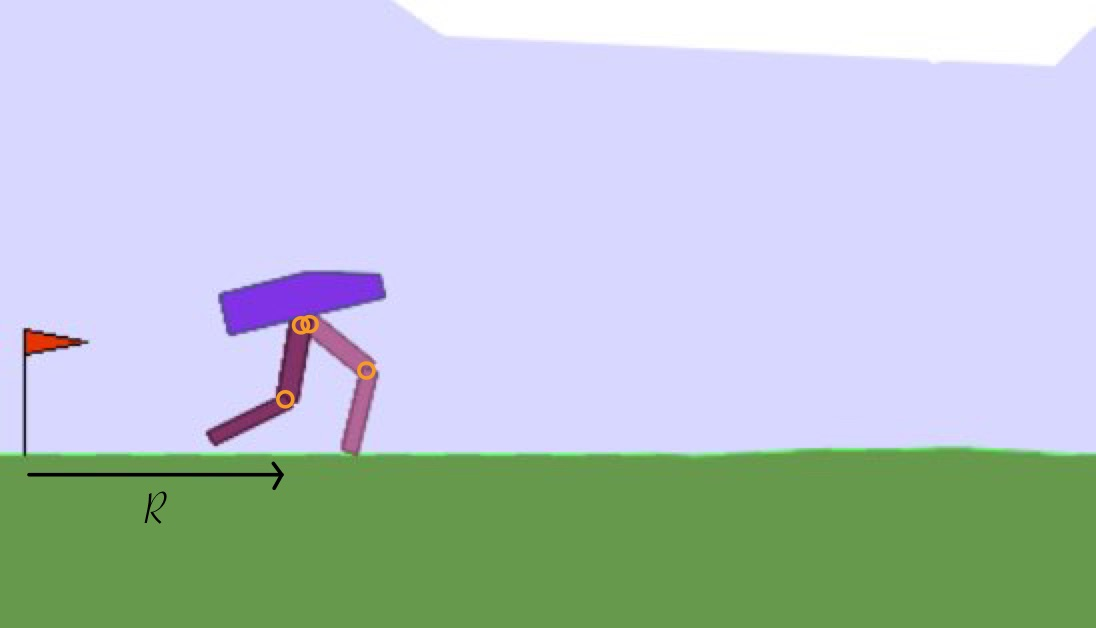
\includegraphics[width=0.45\textwidth]{BipdalWalker-1.jpg} % Passe den Dateinamen und Pfad an
    \caption{Bipedal Walker Environment}
    \label{fig:bwe}
\end{figure}

\noindent The simulation provides an approximation of bipedal locomotion dynamics and includes the following components \cite{pylessons2021bipedalwalker}:

\begin{itemize}
    \item State Space: A 24-dimensional vector representing the robot’s positional and velocity data, joint angles, and foot-ground contact information.
    \item Action Space: A 4-dimensional continuous vector with values in the range [-1,1], representing the torque applied to the four joints (hip and knee for both legs).
    \item Reward Function: The reward is composed of multiple elements: \begin{itemize}
        \item Positive reward for forward movement.
        \item Penalty for energy consumption (high torque usage).
        \item Penalty for falls.
        % \item A terminal reward of +300 when reaching the goal
    \end{itemize}
    
\end{itemize}

\subsubsection{Specific Challenges}
The BipedalWalker environment poses several challenges that make it a demanding benchmark for continuous control algorithms.

\begin{itemize}
    \item Instability: Maintaining dynamic balance is a non-trivial control problem.
    \item Sparse Rewards: Delayed and infrequent reward signals complicate exploration.
    \item Long-Term Planning: The agent must plan multiple steps ahead to develop a stable walk.
    \item High Dimensionality: The combination of a large state and action space requires function approximation.
\end{itemize}

\subsubsection{Training Parameters}

\newacronym{SB3}{SB3}{Stable Baselines 3}

In the experiments we used the \gls{SB3} \cite{stablebaselines3docs2023} library, which provides standardized and efficient implementations of various continuous control algorithms. To ensure a fair comparison, all three algorithms (\gls{DDPG}, \gls{PPO}, and \gls{SAC}) were trained using identical or analogous hyperparameters. The exact hyperparameter configurations used in the implementation are available at our Github Repository \cite{kreil2025github}. The shared hyperparameters are:
\begin{itemize}
    \item Learning rate: $3 \times 10^{-4}$
    \item Discount factor ($\gamma$): $0.99$
    \item Policy: MlpPolicy
\end{itemize}

\noindent For each of the three algorithms, we conducted 5 separate training runs with identical hyperparameters but different random seeds to ensure reliability of results and enable statistical comparability.

\subsubsection{Network Architecture}

All algorithms use the default MlpPolicy from \gls{SB3}, resulting in comparable network structures.

\subsubsection{Evaluation Metrics}

The following metrics were used to compare performance:

\begin{itemize}
    \item Training efficiency: Number of environment interactions required to achieve stable performance.
    \item Stability: Variance in performance across different training runs.
    \item Training Time: The actual wall-clock time required to train the agent.
\end{itemize}

\subsection{Results and Analysis}

\subsubsection{Learning Curves}

\begin{figure}[h] % Use figure* for full-width in twocolumn
    \centering
    \includegraphics[width=0.45\textwidth]{Comparison_of_algorithms.png} % Passe den Dateinamen und Pfad an
    \caption{Learning curves for \gls{DDPG}, \gls{PPO}} and \gls{SAC}
    \label{fig:algo_comperison}
\end{figure}

\noindent The learning dynamics vary significantly across the three algorithms, with the shaded regions in Figure \ref{fig:algo_comperison} representing the standard deviation across all five runs with different random seeds:

\begin{itemize}
    \item \gls{DDPG} (blue): Displays the slowest convergence and only attains \textasciitilde0 reward points at its best, followed by performance decline, which indicates serious stability issues.
    \item \gls{PPO} (green): Converges more slowly, reaching \textasciitilde180 reward points after \textasciitilde400,000 timesteps, with greater fluctuations during training.
    \item \gls{SAC} (red): Converges the fastest and reaches a stable performance level of \textasciitilde280 reward points after \textasciitilde300,000 timesteps.
\end{itemize}

\begin{table}[h]
\scriptsize
\centering
\begin{tabular}{@{}p{1.4cm}p{2.5cm}p{1.2cm}p{2.4cm}@{}}
\toprule
\textbf{Algorithm} & \textbf{Convergence Speed} & \textbf{MaxReward}\\
\midrule
\gls{DDPG} & Low (>500k steps)                  & \textasciitilde0\\
\gls{PPO}  & Medium (\textasciitilde400k steps) & \textasciitilde200\\
\gls{SAC}  & High (\textasciitilde300k steps)   & \textasciitilde300\\

\bottomrule
\end{tabular}
\caption{Comparison of Convergence Speed and Stability}
\end{table}

\noindent \gls{SAC} achieves the fastest convergence, attributed to its off-policy nature and entropy regularization, which promotes broader exploration and more effective reuse of experience \cite{haarnoja2018softactorcriticoffpolicymaximum}. It also demonstrates the most consistent improvements with the lowest variance. \gls{PPO} exhibits moderate fluctuations, while \gls{DDPG} shows consistent underperformance and instability.

\subsubsection{Training Time}

\noindent All reinforcement learning algorithms were trained on a standard laptop computer equipped with an AMD Ryzen 5 5600H (6 cores, 12 threads, 3.3 GHz base clock, 16GB RAM).\\

\begin{table}[h]
\scriptsize
\centering
\begin{tabular}{@{}p{1.4cm}p{2.5cm}p{1.2cm}p{2.4cm}@{}}
\toprule
\textbf{Algorithm} & \textbf{Training Time}\\
\midrule
\gls{DDPG} &  \textasciitilde1.25 hours\\
\gls{PPO}  &  \textasciitilde0.35 hours \\
\gls{SAC}  &  \textasciitilde5.50 hours\\
\bottomrule
\end{tabular}
\caption{Comparison of Training Time}
\end{table}

\noindent Despite \gls{SAC}'s superior sample efficiency, it requires significantly longer wall-clock training time compared to \gls{PPO} and \gls{DDPG}. This is due to \gls{SAC}'s computational complexity from dual Q-networks and automatic entropy tuning, creating higher overhead per step.  In contrast, PPO offers faster training, even without parallelized environments, due to its simpler update mechanism and efficient rollout structure. When parallelized, PPO can further reduce training time dramatically by collecting experience from multiple environments simultaneously. %Meanwhile, \gls{PPO} benefits from its parallelizable structure , processing multiple environments simultaneously and dramatically reducing training time despite requiring more samples.

%\subsection{Discussion of Results}
%\noindent The experimental results provide clear insights into the performance characteristics of these three popular continuous control algorithms when applied to the BipedalWalker task.

%\subsubsection{Which Algorithm is Most Suitable for Bipedal Walking?}
%Based on our experiments using standard SB3 configurations, SAC emerges as the most suitable algorithm for the BipedalWalker task. It achieves superior performance with the highest and most stable reward (~300 points). It has the fastest convergenc (it reaches this performance level within ~200,000 timesteps) and has the best training stability. PPO is a good alternative, achieving similar performance (~270 points) after more interactions (~300,000 timesteps), but with more fluctuations. DDPG consistently underperforms and suffers from instability.

\subsubsection{Theoretical Explanations for Performance Differences}
\begin{itemize}
    \item \gls{SAC} vs. \gls{DDPG}: \gls{SAC}'s entropy promotes better exploration and avoids early convergence to poor strategies, which is useful for complex tasks \cite{haarnoja2018softactorcriticoffpolicymaximum}.
    \item \gls{SAC} vs. \gls{PPO}: \gls{SAC} is off-policy and reuses past experiences, making it more sample-efficient. \gls{PPO}, being on-policy, learns only from recent data \cite{schulman2017proximalpolicyoptimizationalgorithms}.
    \item \gls{PPO} vs. \gls{DDPG}: \gls{PPO} offers more stable training through controlled policy updates \cite{schulman2017proximalpolicyoptimizationalgorithms}. \gls{DDPG} explores less due to its deterministic nature.
\end{itemize}

\subsubsection{No Hyperparameter Tuning}
All experiments mostly used default \gls{SB3} settings, simulating practical conditions where extensive tuning is infeasible. Under these constraints:
\begin{itemize}
    \item \gls{SAC} performs robustly, benefiting from automatic entropy tuning.
    \item \gls{PPO} shows solid performance but may improve with tuned entropy coefficients. %set to 0.0 here
    \item \gls{DDPG} appears most sensitive to parameter choices and would likely benefit from tuning.
\end{itemize}
This suggests that \gls{SAC} is well suited for real-world applications with limited tuning capacity, a key advantage for robotics and control use cases.





\section{Conclusion}

%\subsection{Summary of Key Findings}
%In the BipedalWalker environment, SAC demonstrated superior performance in convergence speed, stability, and final rewards, confirming its effectiveness for continuous control tasks \cite{haarnoja2018softactorcriticoffpolicymaximum}. While SAC is sample-efficient but computationally demanding, PPO offers robust and scalable training, and DDPG struggles without careful tuning. \\

%\noindent Based on our findings, SAC is the preferred choice for tasks requiring data efficiency and robust control, such as real-world robotics applications. PPO, on the other hand, offers stable and scalable training, making it effective in simulated environments that support parallelization. DDPG, while conceptually simple, is highly sensitive to hyperparameters and prone to instability. It should therefore only be used when extensive tuning is feasible.

%\subsection{Summary of Key Findings}
Our comparison of \gls{DDPG}, \gls{PPO}, and \gls{SAC} algorithms on the BipedalWalker-v3 environment reveals valuable insights for reinforcement learning users. \gls{SAC} demonstrated superior performance across all key metrics: faster convergence (stable performance in \textasciitilde300,000 environment interactions), higher final performance (\textasciitilde300 reward points), and greater consistency across multiple runs. These results confirm \gls{SAC}'s effectiveness for continuous control tasks and align with previous findings in the literature.\\

\noindent Without any hyperparameter tuning, our implementation achieves competitive results compared to current state-of-the-art performance on this environment (approximately 300-320 reward points in recent benchmarks).\\ % The performance differences stem from fundamental design choices: SAC's entropy regularization mechanism enables effective exploration while its off-policy learning allows efficient use of past experiences. PPO's conservative policy updates provide stability but limit sample efficiency, while DDPG's deterministic approach proves inadequate for the complex exploration requirements of bipedal locomotion without careful tuning.

\noindent These findings translate into practical recommendations for algorithm selection:

\begin{itemize}
    \item \gls{SAC} is preferred for tasks requiring data efficiency and robust control, such as real-world robotic applications where data collection is expensive and tuning opportunities limited.
    \item \gls{PPO} offers stable and scalable training, making it effective in simulated environments supporting parallelization, particularly where stability is crucial.
    \item \gls{DDPG}, while conceptually simple, is highly sensitive to hyperparameters and prone to instability, making it suitable only when extensive tuning is feasible or for simpler control tasks.
\end{itemize}

\noindent It should be noted that our results are limited to a single environment and may not fully generalize to other continuous control tasks with different dynamics. In addition, all algorithms were evaluated without hyperparameter tuning, which may have particularly impacted \gls{DDPG}'s performance. Nonetheless, they provide practical guidance for algorithm selection in resource-constrained settings.

%\subsection{Future Research Directions}

%Future progress in continuous control will likely be driven by several key research directions. Model-based reinforcement learning promises to improve sample efficiency by incorporating learned dynamics into decision making. Hierarchical approaches, which break down locomotion into simpler subtasks like balance and forward movement, may lead to more scalable and interpretable control. Multi-task and transfer learning could enable agents to generalize better across different environments by reusing acquired knowledge.Integrating prior knowledge, such as physics models or expert demonstrations, could significantly accelerate training and improve performance in complex tasks.

% \section{Methods}

% Maecenas sed ultricies felis. Sed imperdiet dictum arcu a egestas. 
% \begin{itemize}
% \item Donec dolor arcu, rutrum id molestie in, viverra sed diam
% \item Curabitur feugiat
% \item turpis sed auctor facilisis
% \item arcu eros accumsan lorem, at posuere mi diam sit amet tortor
% \item Fusce fermentum, mi sit amet euismod rutrum
% \item sem lorem molestie diam, iaculis aliquet sapien tortor non nisi
% \item Pellentesque bibendum pretium aliquet
% \end{itemize}
% \blindtext % Dummy text

% Text requiring further explanation\footnote{Example footnote}.

%------------------------------------------------

% \section{Results}

% \begin{table}
% \caption{Example table}
% \centering
% \begin{tabular}{llr}
% \toprule
% \multicolumn{2}{c}{Name} \\
% \cmidrule(r){1-2}
% First name & Last Name & Grade \\
% \midrule
% John & Doe & $7.5$ \\
% Richard & Miles & $2$ \\
% \bottomrule
% \end{tabular}
% \end{table}

% \blindtext % Dummy text

% \begin{equation}
% \label{eq:emc}
% e = mc^2
% \end{equation}

% \blindtext % Dummy text

% %------------------------------------------------

% \section{Discussion}

% \subsection{Subsection One}

% A statement requiring citation \cite{doi:10.1126/science.aar6404}.
% \blindtext % Dummy text

% \subsection{Subsection Two}

% \blindtext % Dummy text

%----------------------------------------------------------------------------------------
%	REFERENCE LIST
%----------------------------------------------------------------------------------------
\bibliographystyle{abbrv} % "abbrv" reference style
\bibliography{references} % Entries are in the refs.bib file

%----------------------------------------------------------------------------------------

\end{document}
